% Created 2025-06-24 Tue 10:50
% Intended LaTeX compiler: lualatex
\documentclass[xcolor=table,10pt,aspectratio=169]{beamer}

\RequirePackage[l2tabu,orthodox]{nag}            %% Warn about obsolete commands and packages
\RequirePackage{amsmath,amsfonts,amssymb,amsthm} %% Math
\RequirePackage{ifpdf,ifxetex,ifluatex}          %% Detect XeTeX and LuaTeX
\RequirePackage{xspace}
\RequirePackage{graphicx}
\RequirePackage{comment}
\RequirePackage{url}
\RequirePackage{relsize}
\RequirePackage{booktabs}
\RequirePackage{tabularx}
\RequirePackage[normalem]{ulem}
\ifluatex%
\else%
  \RequirePackage[all]{xy}
\fi%
\RequirePackage{etoolbox}
\RequirePackage{csquotes}
\RequirePackage[export]{adjustbox}

\RequirePackage{silence}
\WarningsOff[microtype]
\WarningFilter{microtype}{Unknown slot}

% https://tex.stackexchange.com/questions/64459/overfull-vbox-warning-disable
\vfuzz=30pt
\hfuzz=30pt


%%%
%%% Code Listings
%%%

\RequirePackage{listings}
\lstdefinelanguage{Sage}[]{Python}{morekeywords={True,False,sage,cdef,cpdef,ctypedef,self},sensitive=true}

\lstset{frame=none,
  showtabs=False,
  showspaces=False,
  showstringspaces=False,
  commentstyle={\color{gray}},
  keywordstyle={\color{mLightBrown}\textbf},
  stringstyle ={\color{mDarkBrown}},
  frame=single,
  basicstyle=\tt\scriptsize\relax,
  backgroundcolor=\color{gray!190!black},
  inputencoding=utf8,
  literate={…}{{\ldots}}1,
  belowskip=0.0em,
}

\makeatletter
\patchcmd{\@verbatim}
  {\verbatim@font}
  {\verbatim@font\scriptsize}
  {}{}
\makeatother


%%%
%%% Pseudocode
%%%

\let\nl\undefine
\let\procedure\relax
\let\endprocedure\relax
\usepackage{algorithm2e}

%%%
%%% Tikz
%%%

\RequirePackage{tikz,pgfplots}
\pgfplotsset{compat=newest}

\usetikzlibrary{calc}
\usetikzlibrary{arrows}
\usetikzlibrary{automata}
\usetikzlibrary{positioning}
\usetikzlibrary{decorations.pathmorphing}
\usetikzlibrary{backgrounds}
\usetikzlibrary{fit,}
\usetikzlibrary{shapes.symbols}
\usetikzlibrary{chains}
\usetikzlibrary{shapes.geometric}
\usetikzlibrary{shapes.arrows}
\usetikzlibrary{graphs}

%% Cache but disable by default

\usetikzlibrary{external}
\tikzset{external/export=false}

\definecolor{DarkPurple}{HTML}{332288}
\definecolor{DarkBlue}{HTML}{6699CC}
\definecolor{LightBlue}{HTML}{88CCEE}
\definecolor{DarkGreen}{HTML}{117733}
\definecolor{DarkRed}{HTML}{661100}
\definecolor{LightRed}{HTML}{CC6677}
\definecolor{LightPink}{HTML}{AA4466}
\definecolor{DarkPink}{HTML}{882255}
\definecolor{LightPurple}{HTML}{AA4499}
\definecolor{DarkBrown}{HTML}{604c38}
\definecolor{DarkTeal}{HTML}{23373b}
\definecolor{LightBrown}{HTML}{EB811B}
\definecolor{LightGreen}{HTML}{14B03D}
\definecolor{DarkOrange}{HTML}{FFDD00}

\pgfplotsset{width=1.0\textwidth,
  height=0.6\textwidth,
  cycle list={%
    solid,LightGreen,thick\\%
    dotted,LightRed,very thick\\%
    dashed,DarkBlue,thick\\%
    dashdotted,DarkPink,thick\\%
    dashdotdotted,LightGreen,thick\\%
    loosely dotted,very thick\\%
    loosely dashed,DarkBlue,very thick\\%
    loosely dashdotted,DarkPink,very thick\\%
    \\%
    DarkBrown,thick\\%
  },
  legend pos=north west,
  legend cell align={left}}

\pgfplotsset{select coords between index/.style 2 args={
    x filter/.code={
        \ifnum\coordindex<#1\def\pgfmathresult{}\fi
        \ifnum\coordindex>#2\def\pgfmathresult{}\fi
    }
}}

\setlength{\marginparwidth}{2cm}
\pgfplotsset{compat=1.18}

%%%
%%% SVG (Inkscape)
%%%

\ifpdf% 
\providecommand{\executeiffilenewer}[3]{%
  \ifnum\pdfstrcmp{\pdffilemoddate{#1}}%
    {\pdffilemoddate{#2}}>0%
    {\immediate\write18{#3}}
  \fi%
}
\else%
\providecommand{\executeiffilenewer}[3]{%
  {\immediate\write18{#3}} % hack
}
\fi%

\providecommand{\includesvg}[2][1.0\textwidth]{%
 \executeiffilenewer{#1.svg}{#1.pdf}%
 {inkscape -z -D --file=#2.svg --export-pdf=#2.pdf --export-latex --export-area-page}%
 \def\svgwidth{#1} 
 \input{#2.pdf_tex}%
} 

%%%
%%% Attachments
%%%

\RequirePackage{embedfile}


%%%
%%% Metropolis Theme
%%%

\usetheme{metropolis}
\metroset{color/block=fill}
\metroset{numbering=none}
\metroset{outer/progressbar=foot}
\metroset{titleformat=smallcaps}

\setbeamercolor{description item}{fg=mLightBrown}
\setbeamerfont{footnote}{size=\scriptsize}
\setbeamercolor{example text}{fg=mDarkBrown}
\setbeamercolor{block title alerted}{fg=white, bg=mDarkBrown}
\setbeamerfont{alerted text}{series=\ifmmode\boldmath\else\bfseries\fi}

\renewcommand*{\UrlFont}{\ttfamily\relax}

%%%
%%% UTF-8 & Fonts
%%% 

% \RequirePackage{unicodesymbols} % after metropolis which loads fontspec

\ifboolexpr{bool{xetex} or bool{luatex}}{%
\setmonofont[BoldFont={Cousine Bold},
             ItalicFont={Cousine Italic},
             BoldItalicFont={Cousine Bold Italic},
             Scale=0.9]{Cousine}             
}{%
}

%%%
%%% BibLaTeX
%%%

\RequirePackage[backend=bibtex,
            style=alphabetic,
            maxnames=8,maxbibnames=8,maxalphanames=8,
            citestyle=alphabetic]{biblatex}

\bibliography{local.bib,abbrev3.bib,crypto_crossref.bib,rfc.bib,jacm.bib,dcc.bib}

\setbeamertemplate{bibliography item}[text]
% https://tex.stackexchange.com/questions/683533/beamer-theme-metropolis-does-not-allow-different-font-size-for-fullcite
\setbeamerfont{bibliography entry title}{size=}
\setbeamerfont{bibliography entry author}{size=}
\setbeamerfont{bibliography entry location}{size=}
\setbeamerfont{bibliography entry note}{size=}

\DeclareFieldFormat{title}{\alert{#1}}
\DeclareFieldFormat[book]{title}{\alert{#1}}
\DeclareFieldFormat[thesis]{title}{\alert{#1}}
\DeclareFieldFormat[inproceedings]{title}{\alert{#1}}
\DeclareFieldFormat[incollection]{title}{\alert{#1}}
\DeclareFieldFormat[article]{title}{\alert{#1}}
\DeclareFieldFormat[misc]{title}{\alert{#1}}

%%% 
%%% Microtype
%%%

\IfFileExists{upquote.sty}{\RequirePackage{upquote}}{}
%% https://github.com/schlcht/microtype/issues/43
%% \IfFileExists{microtype.sty}{\RequirePackage{microtype}}{}
%% \IfFileExists{microtype.sty}{\PassOptionsToPackage{verbose=silent}{microtype}}{}

\setlength{\parindent}{0pt}                   %%
\setlength{\parskip}{6pt plus 2pt minus 1pt}  %%
\setlength{\emergencystretch}{3em}            %% prevent overfull lines
\setcounter{secnumdepth}{0}                   %%

%%%
%%% Maths
%%%

\DeclareMathOperator{\Vol}{Vol}
\DeclareMathOperator{\vol}{vol}
\DeclareMathOperator{\GH}{GH}
\renewcommand{\vec}[1]{\ensuremath{\mathbf{#1}}\xspace}
\newcommand{\norm}[1]{\left\lVert#1\right\rVert}
\providecommand{\mat}[1]{\ensuremath{\vec{#1}}\xspace}
\providecommand{\ring}[0]{\ensuremath{\mathcal{R}}\xspace}


\usepackage{amsmath}
\usepackage{fontspec}
\usepackage{graphicx}
\usepackage{longtable}
\usepackage{wrapfig}
\usepackage{rotating}
\usepackage[normalem]{ulem}
\usepackage{capt-of}
\usepackage{hyperref}
\usepackage{booktabs}
\usepackage{newunicodechar}
\usepackage[notions,operators,sets,keys,ff,adversary,primitives,complexity,asymptotics,lambda,landau,advantage]{cryptocode}
\usepackage[capitalize]{cleveref}
\usepackage[,]{stmaryrd}
\usepackage[english]{babel}
\usepackage{xspace}
\usepackage{units}
\usepackage{nicefrac}
\usepackage{gensymb}
\usepackage{amsthm}
\usepackage{amsmath}
\usepackage{amssymb}
\usepackage{xcolor}
\usepackage{listings}
\usepackage[color=cyan!0!magenta!4!yellow!16]{todonotes}
% \tikzset{external/export=true}
\providecommand{\ring}[0]{\ensuremath{\mathcal{R}}\xspace}
\PassOptionsToPackage{british}{babel}
\usetheme{default}
\author{Martin R. Albrecht}
\date{24 June 2025}
\title{Lattices give us KEMs and FHE, but where are the efficient lattice PETs?}
\subtitle{By Example of (Verifiable) Oblivious PRFs}
\hypersetup{
pdfauthor={Martin R. Albrecht},
pdftitle={Lattices give us KEMs and FHE, but where are the efficient lattice PETs?},
pdfkeywords={},
pdfsubject={},
pdfcreator={Emacs 30.1 (Org mode 9.7.30)},
pdflang={English},
colorlinks,
citecolor=gray,
filecolor=gray,
linkcolor=gray,
urlcolor=gray
}
\begin{document}

\maketitle
\begin{frame}{Outline}
\tableofcontents
\end{frame}

\section{LWE and DH}
\label{sec:orgc131ca1}
\begin{frame}[label={sec:org29b5b28}]{On the one hand, on the other hand}
\begin{columns}[t]
\begin{column}{0.5\columnwidth}
\textbf{Bottom of the Stack:}

\begin{itemize}
\item Kyber (KEM)
\item Dilithium (Signature)
\item Falcon (Signature)
\end{itemize}
\end{column}
\begin{column}{0.5\columnwidth}
\textbf{Top of the Stack:}

\begin{itemize}
\item FHE \cite{PhD:Gentry09,ITCS:BraGenVai12,JC:CGGI20,C:GenSahWat13}
\item iO \cite{FOCS:GGHRSW13,EC:BDGM20}
\item FE \cite{EC:SahWat05,TCC:BonSahWat11}
\end{itemize}
\end{column}
\end{columns}
\end{frame}
\begin{frame}[label={sec:org3af5d3c}]{Somewhat efficient}
\begin{columns}[t]
\begin{column}{0.5\columnwidth}
\textbf{RSA 2048}

\begin{center}
\begin{tabular}{lr}
\toprule
Key generation & \(\approx\) 130,000,000 cycles\\
Encapsulation & \(\approx\) 20,000 cycles\\
Decapsulation & \(\approx\) 2,700,000 cycles\\
Ciphertext & 256 bytes\\
Public key & 256 bytes\\
\bottomrule
\end{tabular}

\end{center}

{\tiny \url{https://bench.cr.yp.to/results-kem.html} }

\textbf{Curve25519}

\begin{center}
\begin{tabular}{lr}
\toprule
Key generation & \(\approx\) 60,000 cycles\\
Key agreement & \(\approx\) 160,000 cycles\\
 & \\
Public key & 32 bytes\\
Key Share & 32 bytes\\
\bottomrule
\end{tabular}

\end{center}

\tiny \url{https://eprint.iacr.org/2015/943}
\end{column}
\begin{column}{0.5\columnwidth}
\textbf{Kyber-768}

\begin{center}
\begin{tabular}{lr}
\toprule
Key generation & ≈  38,000 cycles\\
Encapsulation & ≈  49,000 cycles\\
Decapsulation & ≈  39,000 cycles\\
Ciphertext & 1,088 bytes\\
Public key & 1,184 bytes\\
\bottomrule
\end{tabular}

\end{center}

\tiny \url{https://bench.cr.yp.to/results-kem.html}
\end{column}
\end{columns}
\end{frame}
\begin{frame}[label={sec:org25b77d3}]{The Learning with Errors Problem (LWE)}
Given \((\vec{A},\vec{c})\) with \(\vec{c} \in \ZZ_q^{m}\), \(\vec{A} \in \ZZ_q^{m \times n}\), \(\vec{s} \in \ZZ_q^{n}\) and \alert{small \(\vec{e} \in \ZZ^{m}\)} is

\begin{align*}
\left(\begin{array}{c}
\\
\\
\\ 
\vec{c} \\
\\
\\
\\
\end{array} \right) = \left(
\begin{array}{ccc}
\leftarrow & n & \rightarrow \\
\\
\\ 
& \vec{A} & \\
\\
\\
\\
\end{array} \right) \times \left( \begin{array}{c}
\\
\vec{s} \\
\\
\end{array} \right) \alert{+ \left(
\begin{array}{c}
\\
\\
\\ 
\vec{e} \\
\\
\\
\\
\end{array} 
\right)}
\end{align*}

or \(\vec{c} \sample \mathcal{U}\left(\ZZ_q^{m}\right)\).
\end{frame}
\begin{frame}[label={sec:orgcc6ba71}]{LWE}
\[
\begin{pmatrix}c_{0} \\ c_{1} \\ c_{2} \\ c_{3} \\ c_{4} \\ c_{5} \\ c_{6} \\ c_{7}\end{pmatrix} = 
\left(\begin{array}{rrrrrrrr}
a_{0,0} & a_{0,1} & a_{0,2} & a_{0,3} & a_{0,4} & a_{0,5} & a_{0,6} & a_{0,7}\\
a_{1,0} & a_{1,1} & a_{1,2} & a_{1,3} & a_{1,4} & a_{1,5} & a_{1,6} & a_{1,7}\\
a_{2,0} & a_{2,1} & a_{2,2} & a_{2,3} & a_{2,4} & a_{2,5} & a_{2,6} & a_{2,7}\\
a_{3,0} & a_{3,1} & a_{3,2} & a_{3,3} & a_{3,4} & a_{3,5} & a_{3,6} & a_{3,7}\\
a_{4,0} & a_{4,1} & a_{4,2} & a_{4,3} & a_{4,4} & a_{4,5} & a_{4,6} & a_{4,7}\\
a_{5,0} & a_{5,1} & a_{5,2} & a_{5,3} & a_{5,4} & a_{5,5} & a_{5,6} & a_{5,7}\\
a_{6,0} & a_{6,1} & a_{6,2} & a_{6,3} & a_{6,4} & a_{6,5} & a_{6,6} & a_{6,7}\\
a_{7,0} & a_{7,1} & a_{7,2} & a_{7,3} & a_{7,4} & a_{7,5} & a_{7,6} & a_{7,7}\\
\end{array}\right) \cdot
\begin{pmatrix}s_{0} \\ s_{1} \\ s_{2} \\ s_{3} \\ s_{4} \\ s_{5} \\ s_{6} \\ s_{7}\end{pmatrix} +
\begin{pmatrix}e_{0} \\ e_{1} \\ e_{2} \\ e_{3} \\ e_{4} \\ e_{5} \\ e_{6} \\ e_{7}\end{pmatrix}
\]
\begin{block}{Performance}
Storage: \(\mathcal{O}(n^{2})\); Computation \(\mathcal{O}(n^{2})\)
\end{block}
\end{frame}
\begin{frame}[label={sec:orgbd68151}]{Ring-LWE/Polynomial-LWE}
\[
\begin{pmatrix}c_{0} \\ c_{1} \\ c_{2} \\ c_{3} \\ c_{4} \\ c_{5} \\ c_{6} \\ c_{7}\end{pmatrix} = 
\left(\begin{array}{rrrrrrrr}
\alert{a_{0}} & -a_{7} & -a_{6} & -a_{5} & -a_{4} & -a_{3} & -a_{2} & -a_{1} \\
\alert{a_{1}} & a_{0} & -a_{7} & -a_{6} & -a_{5} & -a_{4} & -a_{3} & -a_{2} \\
\alert{a_{2}} & a_{1} & a_{0} & -a_{7} & -a_{6} & -a_{5} & -a_{4} & -a_{3} \\
\alert{a_{3}} & a_{2} & a_{1} & a_{0} & -a_{7} & -a_{6} & -a_{5} & -a_{4} \\
\alert{a_{4}} & a_{3} & a_{2} & a_{1} & a_{0} & -a_{7} & -a_{6} & -a_{5} \\
\alert{a_{5}} & a_{4} & a_{3} & a_{2} & a_{1} & a_{0} & -a_{7} & -a_{6} \\
\alert{a_{6}} & a_{5} & a_{4} & a_{3} & a_{2} & a_{1} & a_{0} & -a_{7} \\
\alert{a_{7}} & a_{6} & a_{5} & a_{4} & a_{3} & a_{2} & a_{1} & a_{0}
\end{array}\right)\cdot
\begin{pmatrix}s_{0} \\ s_{1} \\ s_{2} \\ s_{3} \\ s_{4} \\ s_{5} \\ s_{6} \\ s_{7}\end{pmatrix} +
\begin{pmatrix}e_{0} \\ e_{1} \\ e_{2} \\ e_{3} \\ e_{4} \\ e_{5} \\ e_{6} \\ e_{7}\end{pmatrix}
\]
\begin{block}{Performance (\(n\) is a power of two)}
Storage: \(\mathcal{O}(n)\); Computation \(\mathcal{O}(n \log n)\)
\end{block}
\end{frame}
\begin{frame}[label={sec:orgbeee0cc}]{Ring-LWE/Polynomial-LWE}
\begin{align*}
\sum_{i=0}^{n-1} c_{i} \cdot X^{i} &= \left(\sum_{i=0}^{n-1} a_{i} \cdot X^{i}\right) \cdot \left(\sum_{i=0}^{n-1} s_{i} \cdot X^{i}\right) + \sum_{i=0}^{8} e_{i} \cdot X^{i} \bmod X^{n} +1\\
c(X) &= a(X) \cdot s(X) + e(X) \bmod \phi(X)
\end{align*}

We write \(\ring \coloneqq \ZZ[X]/\phi(X)\) and \(\ring_{q} \coloneqq \ZZ_{q}[X]/\phi(X)\).

{\footnotesize \fullcite{AC:SSTX09} \par}

{\footnotesize \fullcite{EC:LyuPeiReg10} \par}
\end{frame}
\begin{frame}[label={sec:org7ac3625}]{Convention}
\begin{itemize}
\item I am going to use the Ring-LWE formulation \[c_{i}(X) = a_{i}(X)\cdot s(X) + e_{i}(X)\]
Thus, each sample corresponds to ``\(n\) LWE samples''
\item I will suppress the ``\((X)\)'' in ``\(a(X)\)'' etc.
\item I will assume \(s\) is ``small'' and that the product of two ``small'' things is ``small''.
\item I will write \(\alert{e_{i}}\) to emphasise that \(e_{i}\) is small.
\end{itemize}
\begin{block}{TL;DR: I will write}
\[c_{i} = a_{i}\cdot \alert{s} + \alert{e_{i}}\]
\end{block}
\end{frame}
\begin{frame}[label={sec:org51e35bc}]{DH to Ring-LWE Dictionary}
\begin{center}
\begin{tabular}{ll}
\toprule
DH Land & Ring-LWE Land\\
\midrule
\(g\) & \(a\)\\
\(g^x\) & \(a\cdot {s} + \alert{e}\)\\
 & \\
\(g^x \cdot g^y = g^{x+y}\) & \((a\cdot {s} + \alert{e_0}) + (a \cdot {t} + \alert{e_1}) = a \cdot {(s+t)} + \alert{e'}\)\\
 & \\
\((g^a)^b = (g^b)^a\) & \((a\cdot \alert{s} + \alert{e})\cdot \alert{t} = (a\cdot \alert{s} \cdot \alert{t} + \alert{e} \cdot \alert{t})\)\\
 & \(\approx a\cdot \alert{s} \cdot \alert{t} \approx (a\cdot \alert{t} + \alert{e})\cdot \alert{s}\)\\
 & \\
\((g, g^a, g^b, g^{ab})\) & \((a,\ a\cdot \alert{s} + \alert{e},\ a\cdot \alert{t} + \alert{d},\ a \cdot \alert{s} \cdot \alert{t} + \alert{e'})\)\\
\(\approx_c (g, g^a, g^b, u)\) & \(\approx_c (a,\ a\cdot \alert{s} + \alert{e},\ a\cdot \alert{t} + \alert{d},\ u)\)\\
\bottomrule
\end{tabular}

\end{center}
\end{frame}
\begin{frame}[label={sec:org6d6a974}]{ElGamal \& LPR10}
\textbf{ElGamal}

\begin{description}
\item[{KeyGen}] \(h = g^{s}\)
\item[{Encrypt}] \(d_{0},\ d_{1} = \left({g^{v},\  m \cdot h^{v}}\right)\) for some random \(v\)
\item[{Decrypt}] \(d_{1} / d_{0}^{s} = m \cdot (g^{s})^{v} / (g^{v})^{s} = m\)
\end{description}

\textbf{\cite{EC:LyuPeiReg10}}

\begin{description}
\item[{KeyGen}] \(c = a \cdot \alert{s} + \alert{e}\)
\item[{Encrypt}] \(d_{0}, \ d_{1} = \alert{v} \cdot a + \alert{e'},\ \alert{v} \cdot c + \alert{e''} +\left\lfloor \frac{q}{2} \right\rfloor  \cdot m\)
\item[{Decrypt}] \begin{align*}
\left\lfloor \frac{2}{q} \cdot \left(d_{1} - d_{0} \cdot \alert{s}\right) \right\rceil &= \left\lfloor \frac{2}{q} \cdot \left({\alert{v} \cdot (a \cdot \alert{s} + \alert{e}) + \alert{e''} + \left\lfloor \frac{q}{2} \right\rfloor \cdot m - \left(\alert{v} \cdot a + \alert{e'}\right) \cdot \alert{s}}\right) \right\rceil\\
&= \left\lfloor \frac{2}{q} \cdot \left({\alert{v} \cdot \alert{e} + \alert{e''} + \left\lfloor \frac{q}{2} \right\rfloor  \cdot m - \alert{e'} \cdot \alert{s}}\right) \right\rceil = m\\
\end{align*}
\end{description}
\end{frame}
\section{Follow the Blueprint}
\label{sec:org12db82d}

\begin{frame}[label={sec:org23c4bd3}]{Verifiable Oblivious PRFs}
\procedure{}{%
\textbf{Client} \< \<  \textbf{Functionality} \< \< \textbf{Server}\\
\< \sendmessageright{top=\(m\)} \< \< \sendmessageleft{top=\(k\)} \<\\
\< \< \text{\(c = F_k(m)\)} \< \<\\
\< \sendmessageleft{top=\(c\)} \< \< \sendmessageright{top=\(\bot\)} \<\\
}
\end{frame}
\begin{frame}[label={sec:org1d7d31c}]{Example Applications: Privacy Pass}
\begin{columns}[t]
\begin{column}{0.6\columnwidth}
\textbf{Problem:}

\begin{itemize}
\item Tor users are having a hard time on Cloudflare protected sites
\item They’re constantly asked to solve CAPTCHAs to prove that they’re not bots
\item Want a privacy-preserving way of running reverse Turing test once and re-use later
\end{itemize}
\end{column}
\begin{column}{0.4\columnwidth}
\textbf{Idea:}

\begin{itemize}
\item Solve CAPTCHA
\item Evaluate a VOPRF on a bunch of random points to produce tokens \(F_k(x_i)\)
\item Redeem token by sending \((x_i, F_k(x_i))\)
\end{itemize}
\end{column}
\end{columns}
\vspace{1em}

{\footnotesize \fullcite{PoPETS:DGSTV18} \par}
\end{frame}
\begin{frame}[label={sec:orge5215ee}]{DH-Based OPRF}
\centering
\procedure{}{%
\textbf{Client} \< \< \textbf{Server}\\
\< \sendmessageright*{\text{\(c_x \coloneqq  H(x) \cdot g^{r}\)}} \<\\
\< \sendmessageleft*{\text{\(d_x \coloneqq  c_x^k, c = g^{k}\)}} \<\\
\text{\(d_x/c^r = H(x)^k\)} \< \<\\
}

\[d_x/c^r = c_x^k/c^r = (H(x) \cdot g^{r})^k/(g^k)^r = H(x)^k\]
\end{frame}
\begin{frame}[label={sec:org0bf7ecc}]{``Just take Logs''}
\centering
\procedure{}{%
\textbf{Client} \< \< \textbf{Server}\\
\< \sendmessageright{length=5cm,top=\text{\(c_x \coloneqq  H(x) + a \cdot \alert{r} + \alert{e}\)}} \<\\
\< \sendmessageleft{length=5cm,top=\text{\(d_x \coloneqq c_x \cdot \alert{k} + \alert{e'}, c := a \cdot \alert{k} + \alert{e''}\)}} \<\\
\text{\(\left\lfloor \frac{p}{q} \cdot d_x - c \cdot \alert{r} \right\rceil \)} \< \<\\
}

\begin{align*}
d_x - c \cdot \alert{r}  &= \left(H(x) + a \cdot \alert{r} + \alert{e}\right)\cdot\alert{k} + \alert{e'} - \left(a \cdot \alert{k} + \alert{e''}\right) \cdot \alert{r}\\
                     &= H(x)\cdot\alert{k} + a \cdot \alert{r}\cdot\alert{k} + \alert{e}\cdot\alert{k} + \alert{e'} - a \cdot \alert{k} \cdot \alert{r} - \alert{e''} \cdot \alert{r}\\
                     &= H(x)\cdot\alert{k} + \alert{e}\cdot\alert{k} + \alert{e'}  - \alert{e''} \cdot \alert{r}\\
                     &\approx H(x)\cdot\alert{k} 
\end{align*}
\end{frame}
\begin{frame}[label={sec:org9d5c4fb}]{The Trouble}
\begin{description}
\item[{Trapdoor Friendly}] It is not safe to output \(c_{x} \cdot \alert{k} + \alert{e}\) for some arbitrary \(c_{x}\)
\item[{Noise Leakage}] ``\(\approx\)'' glosses over \(\alert{e}\cdot\alert{k} + \alert{e}'  - \alert{e}'' \cdot \alert{r}\) which depends on \(k\)
\item[{Noise Growth}] ``\(\approx\)'' is not \(=\), how do we arrive at the same value?
\end{description}
\end{frame}
\section{Trapdoor Friendly}
\label{sec:orgbcdfd5b}

\begin{frame}[label={sec:org3e06570}]{The Problem}
\begin{center}
The server has to output \(c_{x} \cdot \alert{k} + \alert{e}'\) for some \(c_x \overset{?}{=}  H(x) + a \cdot \alert{r} + \alert{e}\). This may not be safe.
\end{center}
\end{frame}
\begin{frame}[label={sec:org30ea146},fragile]{Point Validation}
\begin{columns}
\begin{column}[t]{0.5\columnwidth}
\newcommand{\mfi}[1]{\fbox{\includegraphics[width=0.4\paperwidth]{#1}}}
\setlength{\fboxsep}{0pt}
\begin{tikzpicture}
\pgfplotsset{width=\textwidth, height=\textheight}
\only<1->{\node[anchor=north west] at (0,0) {\mfi{point-validation-PKC_ABMSV03.png}};}
\only<2->{\node[anchor=north west] at (0.5,-0.5) {\mfi{point-validation-CCS_AMPS18.png}};}
\node[anchor=north west] at (0.5,-0.5) {\phantom{{\mfi{point-validation-CCS_AMPS18.png}}}};
\end{tikzpicture}
\end{column}
\begin{column}[t]{0.5\columnwidth}
\pause
\pause

\begin{itemize}
\item However, (likely) no ``point validation'' for LWE by the NTRU assumption \cite{NTRU:HPS98}:
\[
  \alert{f}, \alert{g} \sample \ring^{2}: h \coloneqq f/g \approx_{c} \mathcal{U}(\ring_q)
  \]
\item Attack\footnote{assuming \(\alert{f},\alert{g},\alert{k},\alert{e}\) are sufficiently small}:
\begin{enumerate}
\item Sample \(\alert{f},\alert{g} \sample \ring^{2}\) and set \(\Delta \coloneqq  \lceil \sqrt{q} \rceil\)
\item Submit \(a \coloneqq \Delta \cdot f/g\)
\item Receive \(c \coloneqq a \cdot \alert{k} + \alert{e}\) and compute
\end{enumerate}
\begin{align*}
  \alert{g} \cdot c & = \alert{g} \cdot (\Delta \cdot f/g \cdot \alert{k} + \alert{e})\\
  \alert{g} \cdot c & = \Delta \cdot \alert{f} \cdot \alert{k} + \alert{g} \cdot \alert{e}\\
        &\equiv \alert{g} \cdot \alert{e} \bmod \Delta
\end{align*}
\end{itemize}
\end{column}
\end{columns}
\end{frame}
\begin{frame}[label={sec:orgd569696}]{Workaround}
\begin{itemize}
\item The client proves in zero-knowledge that \(c_{x}\) is well-formed: \(c_{x} \coloneqq H(x) + a \cdot \alert{r} + \alert{e}\)
\item This means the client needs to prove the evaluation of \(H(x)\)
\item This is sound, we do not need to treat \(H(x)\) as a Random Oracle
\item This is expensive in terms of bandwidth and computation cost
\begin{itemize}
\item \cite{PKC:ADDS21}: \(\approx\) 128GB per evaluation using \cite{C:YAZXYW19}
\item \cite{AC:AlbGur24}: \(\approx\) 63kB per evaluation using \cite{C:BeuSei23}
\end{itemize}
\end{itemize}
\begin{alertblock}{An Aside}
This NTRU ``attack'' can be used constructively to make proof systems online extractable (e.g. \cite{EC:ADDG24})
\end{alertblock}
\end{frame}
\section{Noise Leakage}
\label{sec:org626fd9c}

\begin{frame}[label={sec:org1cb472a}]{The Problem}
The client learns
\[\alert{e}\cdot\alert{k} + \alert{e}'  - \alert{e}'' \cdot \alert{r}\]
where it chooses \(\alert{e}\) and \(\alert{r}\). 
\begin{block}{The Attack}
Write \(\alert{\vec{a}} \coloneqq (\alert{e}, -\alert{r})\) and \(\alert{\vec{s}} \coloneqq (\alert{k}, \alert{e''})\), then we can rewrite \[\alert{e}\cdot\alert{k} + \alert{e}'  - \alert{e}'' \cdot \alert{r}\]
as \(\alert{\vec{a}} \cdot \alert{\vec{s}} + \alert{e''}\) which is essentially an instance of ``LWE without modular reduction'' \cite{AC:BDEFT18} which is easy.\footnote{The word ``essentially'' does a lot of work here. That is, this is a simplification because \(\alert{e''}\) changes in each invocation and the attacks from \cite{AC:BDEFT18} do not apply as is.}
\end{block}
\end{frame}
\begin{frame}[label={sec:orgf83cf19}]{Solutions}
\begin{description}
\item[{Statistical Noise Drowning}] \(\Vert\alert{e}'\Vert \geq \lambda^{\omega(1)} \cdot \Vert\alert{e}\cdot\alert{k}  - \alert{e}'' \cdot \alert{r}\Vert\) \cite{PKC:ADDS21}
\item[{Rényi Noise Drowning}] \(\Vert\alert{e}'\Vert \geq \poly \cdot \sqrt{Q} \cdot \Vert\alert{e}\cdot\alert{k}  - \alert{e}'' \cdot \alert{r}\Vert\) \cite{AC:AlbGur24}
\begin{itemize}
\item \(Q\) is the number of queries
\item must play a search game instead of a distinguishing game (use ROM)
\end{itemize}
\item[{Computational Assumption}] \(\Vert\alert{e}'\Vert \geq \poly \cdot \sqrt{Q} \cdot \Vert\alert{e}\cdot\alert{k}  - \alert{e}'' \cdot \alert{r}\Vert\) \cite{EPRINT:ESTX24}
\begin{itemize}
\item similar to Hint-(M)LWE, but w/o reduction from (M)LWE
\end{itemize}
\end{description}
\begin{block}{Cost}
Since we require \(q > \Vert\alert{e}'\Vert\) we have that \(q/\Vert \alert{e} \Vert\) -- the ``signal to noise ratio'' of the underlying RLWE samples -- is quite big.  A big signal to noise ratio makes decoding -- i.e. solving LWE -- easier. This requires us to use larger secret dimensions \(n\) to compensate. Bandwidth cost is essentially \(n \log q\).
\end{block}
\end{frame}
\section{Noise Growth}
\label{sec:orgd260c27}

\begin{frame}[label={sec:org46b174e}]{The Problem}
\begin{align*}
H(x)\cdot\alert{k} + \alert{e}\cdot\alert{k} + \alert{e'}  - \alert{e''} \cdot \alert{r}
&\approx H(x)\cdot\alert{k}\\
\left\lceil \frac{2}{q} \cdot \bigg(H(x)\cdot\alert{k} + \alert{e}\cdot\alert{k} + \alert{e'}  - \alert{e''} \cdot \alert{r}\bigg)\right\rfloor
&\overset{?}{=} \left\lceil \frac{2}{q} \cdot \bigg( H(x)\cdot\alert{k} \bigg)\right\rfloor
\end{align*}
\end{frame}
\begin{frame}[label={sec:org593a3e1}]{Rounding}
\centering
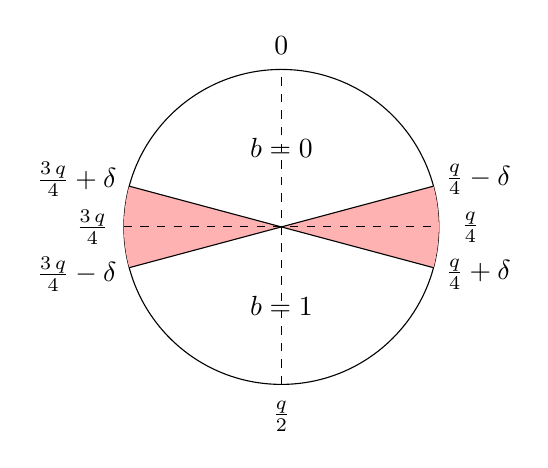
\begin{tikzpicture}
  \draw (0,0) circle (2cm);

  \fill[red!30] (0,0) -- (-15:2cm) arc (-15:15:2cm) -- cycle;
  \fill[red!30] (0,0) -- (165:2cm) arc (165:195:2cm) -- cycle;


  \draw[dashed] (0,-2) -- (0,2);
  \draw[dashed] (-2,0) -- (2,0);
  \draw[rotate=75] (0,-2) -- (0,2);
  \draw[rotate=-75] (0,-2) -- (0,2);

  \node at (0,2.3) {$0$};
  \node at (2.5,0.6) {$\frac{q}{4}-\delta$};
  \node at (2.4,0) {$\frac{q}{4}$};
  \node at (2.5,-0.6) {$\frac{q}{4}+\delta$};
  \node at (0,-2.4) {$\frac{q}{2}$};
  \node at (-2.6,0.6) {$\frac{3\,q}{4}+\delta$};
  \node at (-2.4,0) {$\frac{3\,q}{4}$};
  \node at (-2.6,-0.6) {$\frac{3\,q}{4}-\delta$};

  \node at (0, 1) {$b=0$};
  \node at (0,-1) {$b=1$};

\end{tikzpicture}
\end{frame}
\begin{frame}[label={sec:org317d417}]{Solution Attempt}
\begin{columns}
\begin{column}{0.5\columnwidth}
Make \(q > \poly\) such that the red area is negligibly small.
\begin{block}<2->{Malicious Servers}
This argument works on average but does not work against adversaries that somehow pick \(k\) s.t. \(H(x) \cdot k\) lands in the red area with high probability for some \(x\).
\end{block}
\end{column}
\begin{column}{0.5\columnwidth}
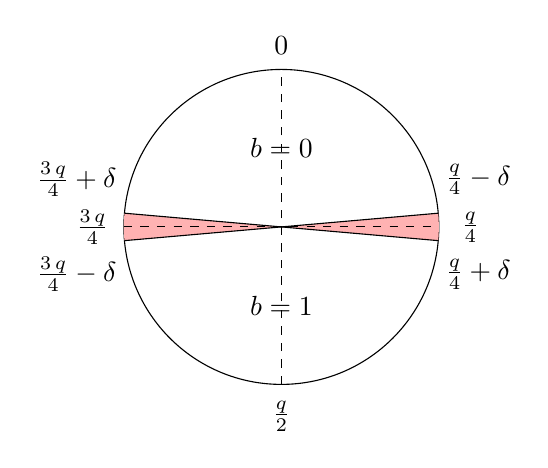
\begin{tikzpicture}
  \draw (0,0) circle (2cm);

  \fill[red!30] (0,0) -- (-5:2cm) arc (-5:5:2cm) -- cycle;
  \fill[red!30] (0,0) -- (175:2cm) arc (175:185:2cm) -- cycle;


  \draw[dashed] (0,-2) -- (0,2);
  \draw[dashed] (-2,0) -- (2,0);
  \draw[rotate=85] (0,-2) -- (0,2);
  \draw[rotate=-85] (0,-2) -- (0,2);

  \node at (0,2.3) {$0$};
  \node at (2.5,0.6) {$\frac{q}{4}-\delta$};
  \node at (2.4,0) {$\frac{q}{4}$};
  \node at (2.5,-0.6) {$\frac{q}{4}+\delta$};
  \node at (0,-2.4) {$\frac{q}{2}$};
  \node at (-2.6,0.6) {$\frac{3\,q}{4}+\delta$};
  \node at (-2.4,0) {$\frac{3\,q}{4}$};
  \node at (-2.6,-0.6) {$\frac{3\,q}{4}-\delta$};

  \node at (0, 1) {$b=0$};
  \node at (0,-1) {$b=1$};


\end{tikzpicture}
\end{column}
\end{columns}
\end{frame}
\begin{frame}[label={sec:orgc922523}]{Solution}
\begin{itemize}
\item Plant a hard SIS instance in each coefficient: 1D-SIS \cite{PKC:ADDS21}
\pause
\begin{itemize}
\item Yes, seriously!
\item This requires \(q \gg 2^{\secpar}\)
\end{itemize}
\pause
\item Change the PRF output to \(H(x) \cdot \alert{k} + H_{2}(x,c_0)\) \cite{AC:AlbGur24}
\begin{itemize}
\item \(H_{2}()\) is some Random Oracle that randomly shifts \(H(x) \cdot \alert{k}\)
\item \(c_{0} \coloneqq a_{0} \cdot \alert{k} + \alert{e_{0}'}\) is a commitment to \(\alert{k}\)
\item The trick is from \cite{USENIX:GKQMS24}
\item \(q \gg \poly\) is sufficient
\end{itemize}
\end{itemize}
\begin{block}{Stuck with a super-polynomial \(q\)}
Big ``signal-to-noise'' ratio, forcing us to increase \(n\), as above.
\end{block}
\end{frame}
\begin{frame}[label={sec:org8fcd566}]{Related: Can't Just Do It™ — NIKE}
NIKE enables Alice and Bob, who know each others’ public keys, to agree on shared key without requiring any interaction \cite{DifHel76}
\begin{itemize}
\item Deployed in \href{https://www.wireguard.com/}{WireGuard} \cite{EPRINT:HNSWZ20} and static DH is also used in e.g. Google’s QUIC.
\item For lattices there are significant barriers \cite{PKC:GKRS20}.
\item Stark contrast to \alert{interactive} key-exchanges or plain public-key encryption
\begin{enumerate}
\item We send along some “hints” that allow to handle the noise
\item secrets are not re-used, allowing us to avoid expensive “well-formedness” proofs
\end{enumerate}
\item \cite{USENIX:GKQMS24} is an instantiation that essentially accepts the super-polynomial modulus
\end{itemize}
\end{frame}
\section{Wrapping Up}
\label{sec:org9559df9}

\begin{frame}[label={sec:orgc251170}]{Realisations of this Blueprint}
\begin{center}
\begin{tabular}{llrrl}
\toprule
Work & Model & 1-time Offline & Online & \(Q\)\\
\midrule
\cite{PKC:ADDS21} & H-H & -- & 2MB & \\
\cite{PKC:ADDS21} & M-M & -- & 128GB & \\
\cite{AC:AlbGur24} & M-M & 114kB & 198kB & \(2^{32}\)\\
\cite{EPRINT:ESTX24} & M-M & 20kB & 159kB & \(2^{32}\)\\
\bottomrule
\end{tabular}

\end{center}

\begin{center}
H: semi-honest, M: malicious
\end{center}
\end{frame}
\begin{frame}[label={sec:orgdeb9b98}]{An Alternative from FHE \cite{EC:ADDG24}}
We do have efficient FHE, indeed FHE ciphertexts are typically \alert{smaller} than the messages exchanged in the schemes discussed above.
\begin{itemize}
\item Simple idea:
\begin{enumerate}
\item Client FHE encrypts \(x\) as \([x]\)
\item Server homomorphically computes PRF using plaintext \(k\) and \([x]\) to obtain \([F_{k}(x)]\)
\item Client FHE decrypts \(F_{k}(x)\)
\end{enumerate}
\item Problem: PRFs need deep circuits, deep circuits are expensive
\item Proposal: Use Dark Matter (weak-)PRF candidate \cite{TCC:BIPSW18} \(\sum \left(\mat{A}\cdot \vec{x} \bmod 2\right) \bmod 3\) where \(\mat{A}\) is the secret key
\item This can be computed with one level of FHE bootstrapping
\end{itemize}
\end{frame}
\begin{frame}[label={sec:orgdd2d8a1}]{Other Round-Optimal Alternatives w/o Trusted Setup}
\begin{small}

\begin{center}
\begin{tabular}{lllrr}
\toprule
Work & Assumption & Model & 1-time Offline & Online\\
\midrule
ADDS21 & (R)LWE+SIS & H-H & - & 2MB\\
ADDS21 & (R)LWE+SIS & M-M & - & 128GB\\
AG24 & (R)LWE+SIS & M-M & 114kB & 198kB\\
ADDG23 & mod(2,3)+lattices & M-H & 2.5MB & 10KB\\
ADDG23 & mod(2,3)+lattices & M-M & 2.5MB & 160KB\\
ESTX24 & iMLWER-RU+MLE+SIS & M-M & 20kB & 159KB\\
APRR24 & mod(2,3) & M-H, pp & 4.75B & 114.5B\\
FOO23 & AES+Garbled Circuits & H-H & - & 6.79MB\\
Basso24 & Higher-Dimensional isogenies & M-M & - & 28.9kB\\
HHM+23 & Isogenies F\textsubscript{p} + lattices + HE OT & H-H & - & 640kB\\
dSP23 & Isogenies F\textsubscript{p} & M-H, pp & 68.4 kB & 384B\\
dSP23 & Isogenies F\textsubscript{p} & M-H, pp & - & 16.38kB\\
\bottomrule
\end{tabular}

\end{center}

\end{small}

\begin{center}
{\footnotesize adapted from \url{https://heimberger.xyz/oprfs.html} \par}
\end{center}
\end{frame}
\begin{frame}[label={sec:org916c2a4},standout]{Fin}
\begin{center}
{\Huge\alert{Thank You}\par}

\url{https://ia.cr/2019/1271}

\url{https://ia.cr/2023/232}

\url{https://ia.cr/2024/1459}
\end{center}
\end{frame}
\begin{frame}[allowframebreaks]{References}
\renewcommand*{\bibfont}{\scriptsize}
\printbibliography[heading=none]
\end{frame}
\end{document}
